\documentclass{article}
\usepackage[utf8]{inputenc}
\usepackage{graphicx}
\title{ADD TITLE}
\date{\today}
\begin{document}
\section{Acquisition Parameters}
\begin{itemize}	\item{\textbf{Particle Name}:VivoTrax}
	\item{\textbf{Particle Manufacturer}:Magnetic Insight}
	\item{\textbf{SPION Lot}:}
	\item{\textbf{SPION Mfg. Date}:}
	\item{\textbf{SPION Core Size}:999}
	\item{\textbf{SPION Hydrodynamic Diameter}:999}
	\item{\textbf{Concentration}:5.5}
	\item{\textbf{Sample Volume}:0.018}
	\item{\textbf{SPION Coating}:}
	\item{\textbf{Notes}:There is a small bubble}
	\item{\textbf{User Name}:Eli Mattingly}
	\item{\textbf{User Location}:Martinos Center, Boston, MA, USA}
	\item{\textbf{Total Acquisition Time (Seconds)}:168.9575}
\end{itemize}
\begin{figure}[h] 
 \centering 
 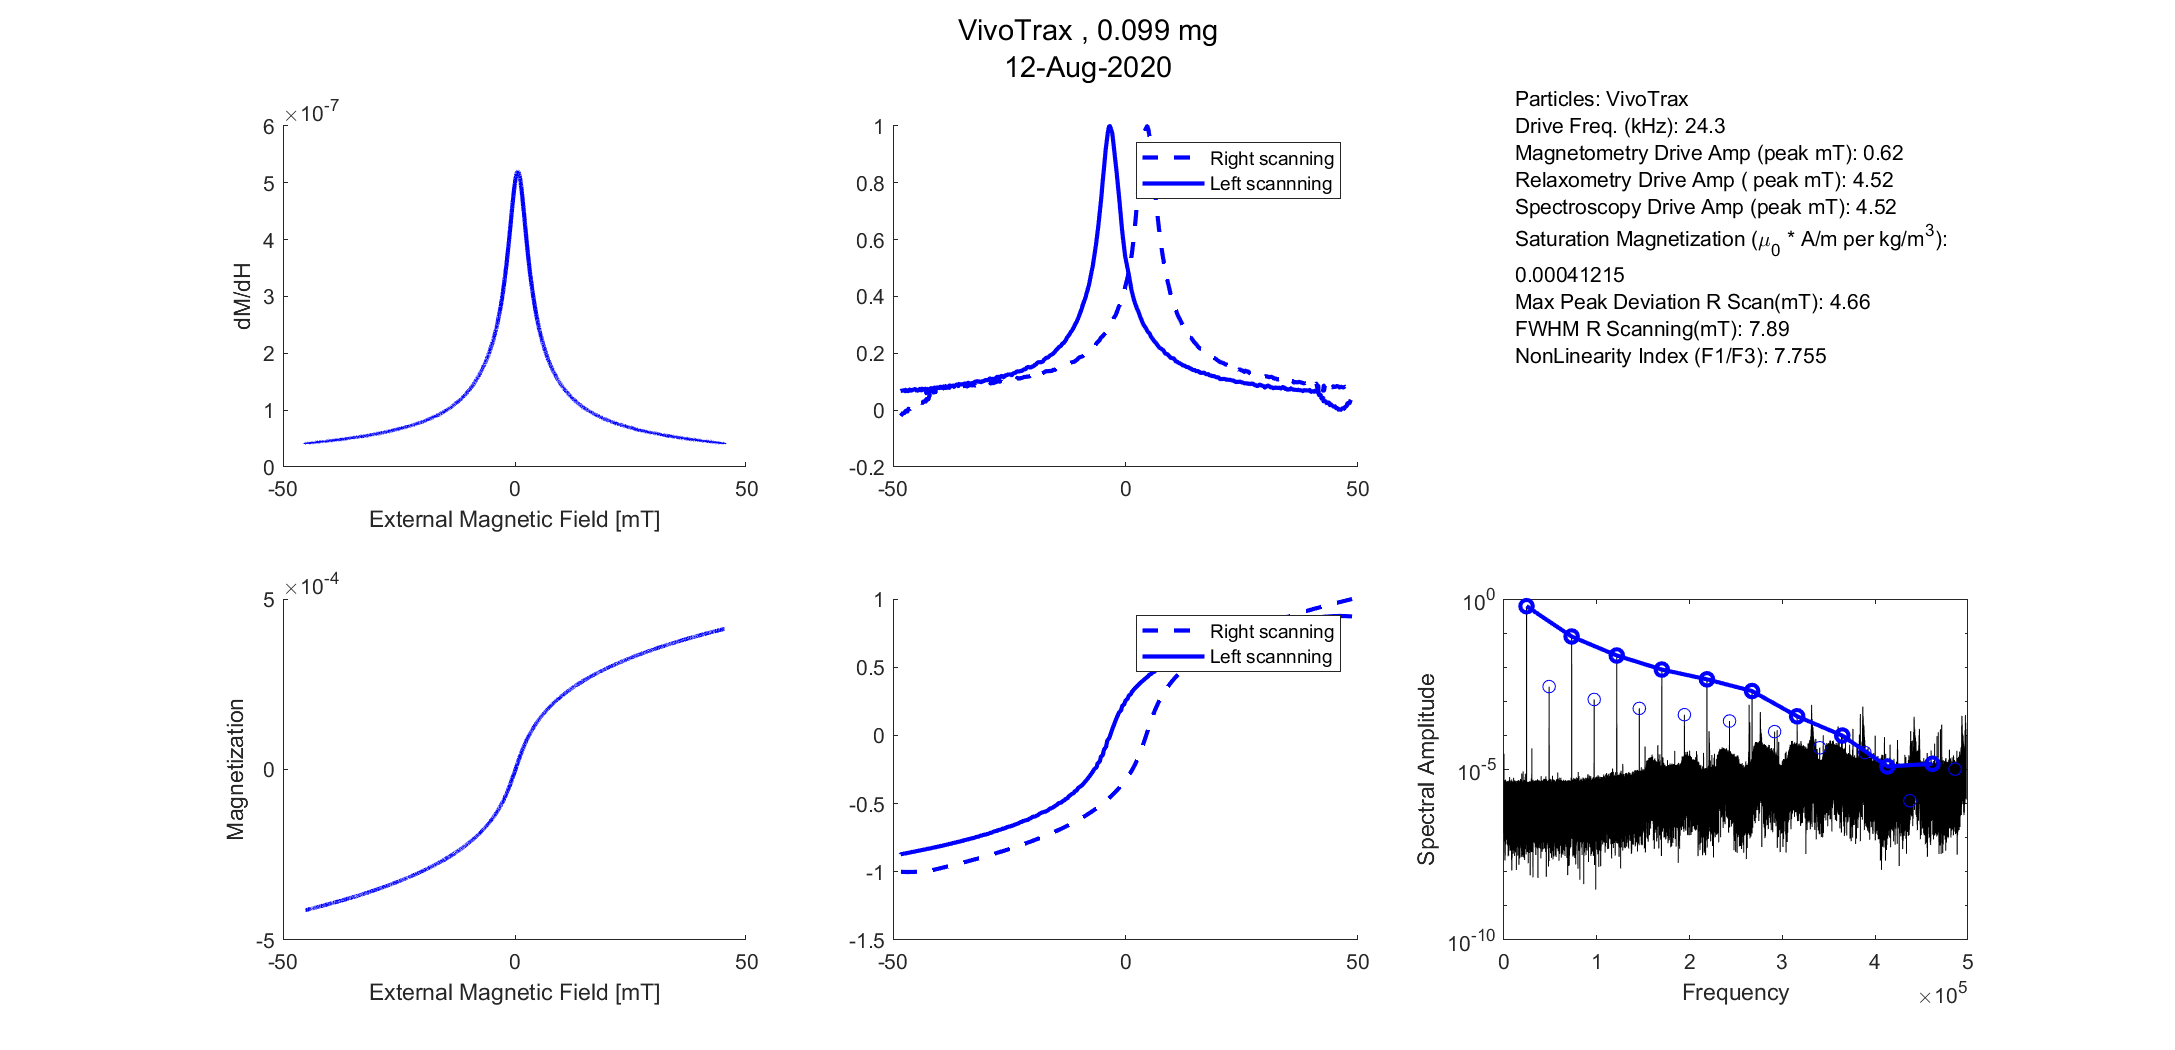
\includegraphics[width=0.9\textwidth]{VivoTrax_12_Aug_2020_CompositeFig.png}
 \caption{A summary of the experiment}
 \end{figure}
\section{Magnetometry}

\begin{itemize}	\item{\textbf{Sampling Freq.}:1000000}
	\item{\textbf{Interpolated Freq.}:996300}
	\item{\textbf{Drive Freq.}:24300}
	\item{\textbf{Bias Freq.}:20}
	\item{\textbf{Bias Waveform Shape}:Sine}
	\item{\textbf{Bias Amplitude (mT)}:45.1291}
	\item{\textbf{Bias Amplitude (Volts)}:1.7495}
	\item{\textbf{Bias Amplifier Name}:RCF IPS700}
	\item{\textbf{Bias Current Monitor Volts Per Amp}:0.04}
	\item{\textbf{Bias Field mT per Amp}:6}
	\item{\textbf{Drive Amplitude (mT)}:0.62081}
	\item{\textbf{Drive Amplitude (Volts)}:0.042764}
	\item{\textbf{Drive Amplifier Name}:OPA549_Single_BoardRev2}
	\item{\textbf{Drive Current Monitor Volts Per Amp}:0.1}
	\item{\textbf{Drive Field mT per Amp}:2}
	\item{\textbf{Power Supply Name}:Tenma 72-7245}
	\item{\textbf{Pre-Amplifier Name}:INA217 V0}
	\item{\textbf{Pre-Amplifier Gain}:100}
	\item{\textbf{Test Time}:2}
	\item{\textbf{Number of Averages}:2}
	\item{\textbf{Saturation Magnetization (\mu_0 * A/m per kg/m^3)}:0.00041215}
\end{itemize}
\begin{figure}[h] 
 \centering 
 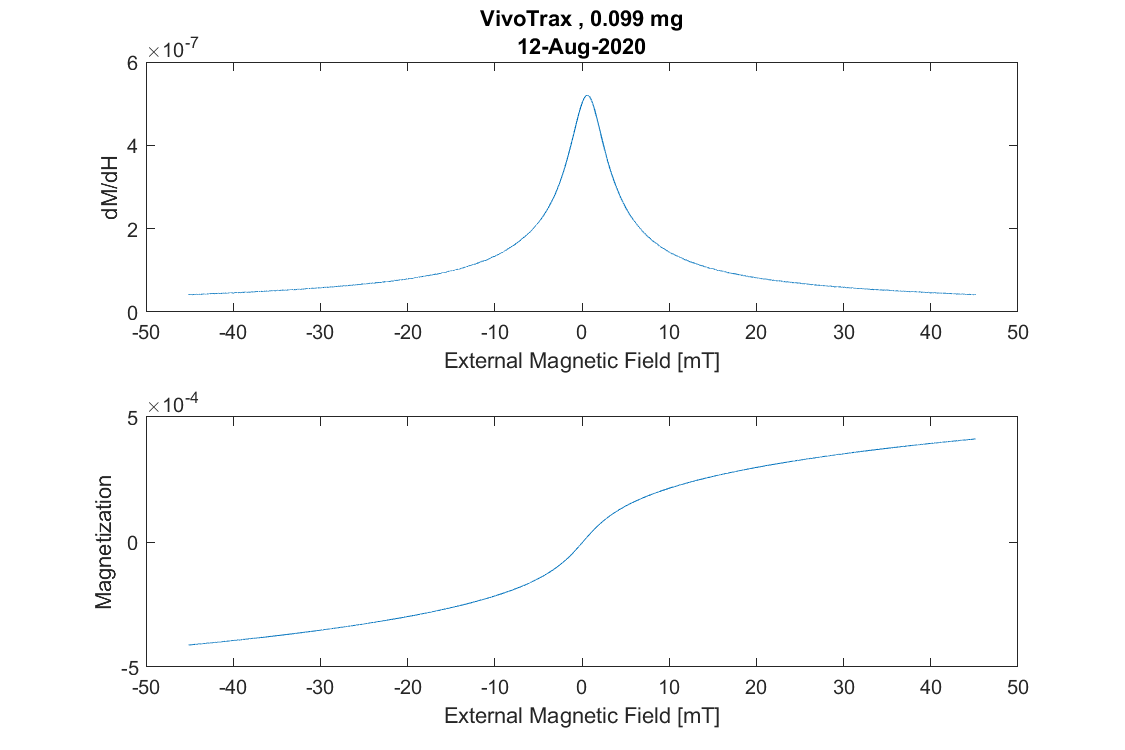
\includegraphics[width=0.9\textwidth]{VivoTrax_12_Aug_2020_MagFig.png}
 \caption{TestCaption for Mag}
 \end{figure}
\section{Relaxometry}
\begin{itemize}
\section{Magnetometry}

\begin{itemize}	\item{\textbf{Sampling Freq.}:1000000}
	\item{\textbf{Interpolated Freq.}:996300}
	\item{\textbf{Drive Freq.}:24300}
	\item{\textbf{Bias Freq.}:20}
	\item{\textbf{Bias Waveform Shape}:Sine}
	\item{\textbf{Bias Amplitude (mT)}:45.033}
	\item{\textbf{Bias Amplitude (Volts)}:1.7495}
	\item{\textbf{Bias Amplifier Name}:RCF IPS700}
	\item{\textbf{Bias Current Monitor Volts Per Amp}:0.04}
	\item{\textbf{Bias Field mT per Amp}:6}
	\item{\textbf{Drive Amplitude (mT)}:4.5202}
	\item{\textbf{Drive Amplitude (Volts)}:0.32073}
	\item{\textbf{Drive Amplifier Name}:OPA549_Single_BoardRev2}
	\item{\textbf{Drive Current Monitor Volts Per Amp}:0.1}
	\item{\textbf{Drive Field mT per Amp}:2}
	\item{\textbf{Power Supply Name}:Tenma 72-7245}
	\item{\textbf{Pre-Amplifier Name}:INA217 V0}
	\item{\textbf{Pre-Amplifier Gain}:100}
	\item{\textbf{Test Time}:2}
	\item{\textbf{Number of Averages}:2}
	\item{\textbf{Max Peak Deviation R Scan(mT)}:4.6556}
	\item{\textbf{Max Peak Deviation L Scan(mT)}:-3.3237}
	\item{\textbf{FWHM R Scanning(mT)}:7.8939}
	\item{\textbf{FWHM L Scanning(mT)}:7.9373}
\begin{figure}[h] 
 \centering 
 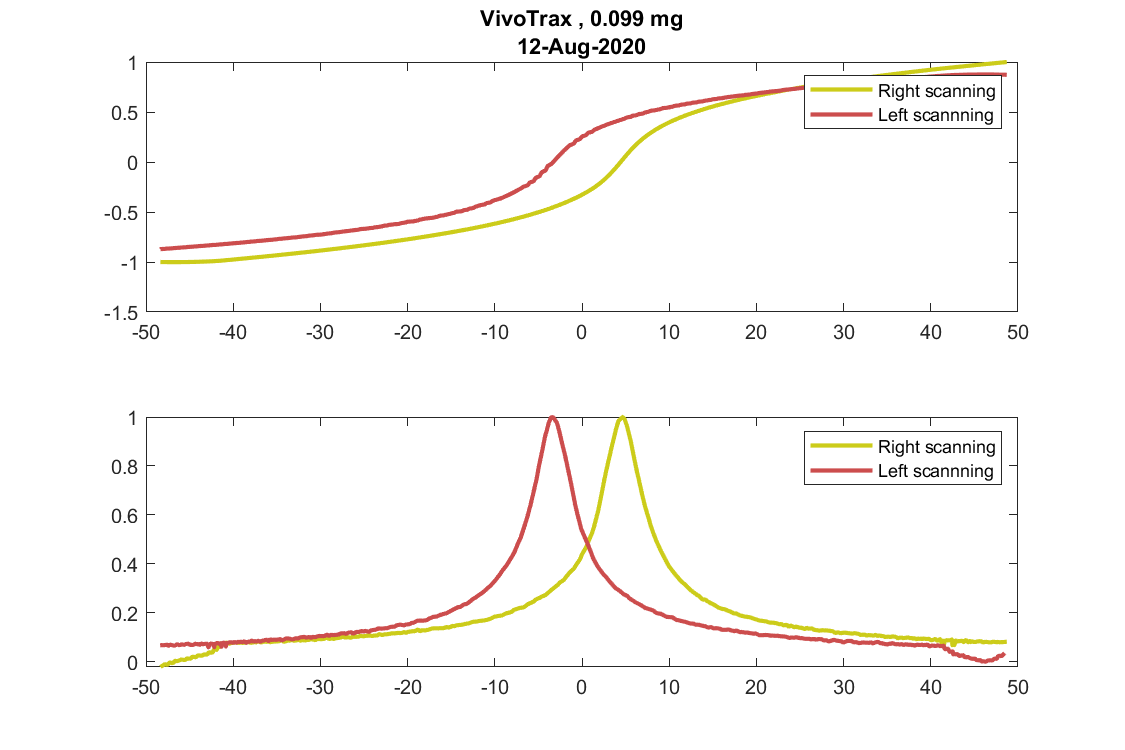
\includegraphics[width=0.9\textwidth]{VivoTrax_12_Aug_2020_RelaxFig.png}
 \caption{Results from the relaxometry experiment}
 \end{figure}\end{itemize}

\section{Spectroscopy}
\begin{itemize}	\item{\textbf{Sampling Freq.}:1000000}
	\item{\textbf{Interpolated Freq.}:996300}
	\item{\textbf{Drive Freq.}:24300}
	\item{\textbf{Drive Amplitude (mT)}:4.5178}
	\item{\textbf{Drive Amplitude (Volts)}:0.32073}
	\item{\textbf{Drive Amplifier Name}:OPA549_Single_BoardRev2}
	\item{\textbf{Drive Current Monitor Volts Per Amp}:0.1}
	\item{\textbf{Drive Field mT per Amp}:2}
	\item{\textbf{Power Supply Name}:Tenma 72-7245}
	\item{\textbf{Pre-Amplifier Name}:INA217 V0}
	\item{\textbf{Pre-Amplifier Gain}:100}
	\item{\textbf{Test Time}:2}
	\item{\textbf{Number of Averages}:2}
	\item{\textbf{NonLinearity Index (F1/F3)}:7.755}
\begin{figure}[h] 
 \centering 
 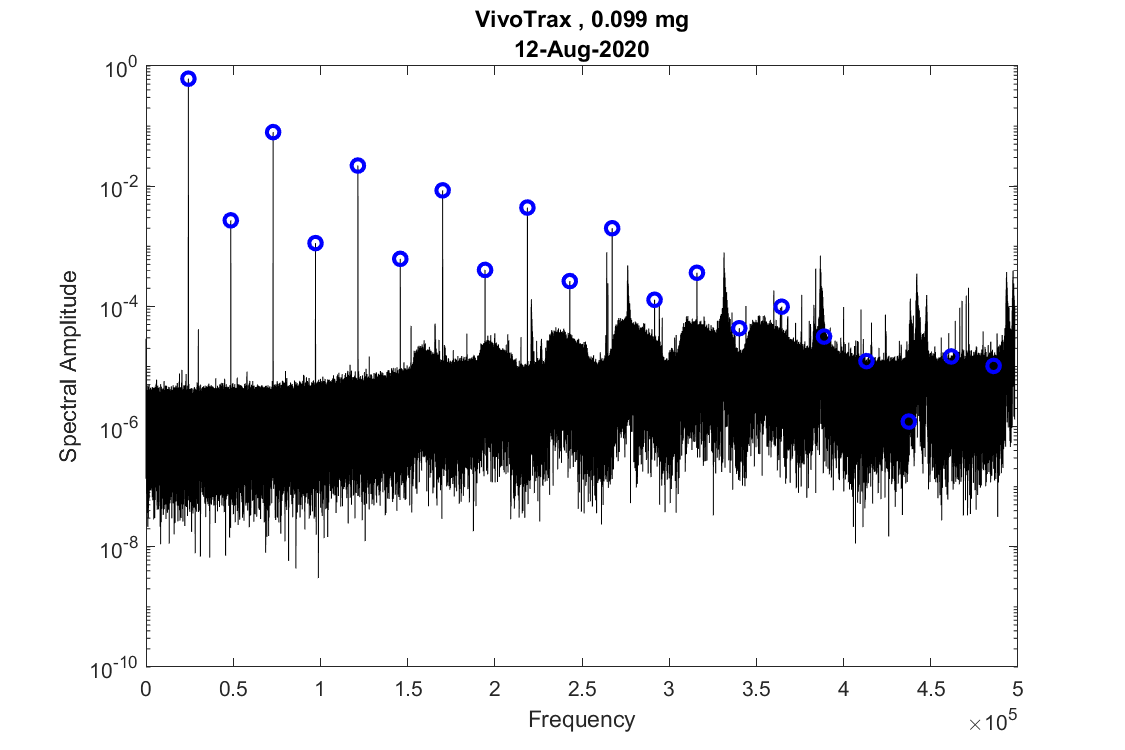
\includegraphics[width=0.9\textwidth]{VivoTrax_12_Aug_2020_SpecFig.png}
 \caption{Results from the spectroscopy}
 \end{figure}\end{itemize}

\end{document}